The language of \textsc{EviL} is evidently modal, and in previous
sections the semantics have largely suggested that there are clear
connections to conventional Kripke semantics.  
In this section, we will demonstrate that every \textsc{EviL} model
corresponds to some highly structured Kripke model, with a minor
modification on the standard definition.  However, it will turn out
that this correspondence is one way - the class of Kripke models for
which \textsc{EviL} is strongly complete do not, in general,
possess corresponding \textsc{EviL} models.

To elucidate my intuition for understanding \textsc{EviL} models as
Kripke models, we would like to return to the visualization technique for
\textsc{EviL} models we introduced in \S\ref{contradictions}.  This
involved, roughly, thinking of the \textsc{EviL} models as 
\emph{posets} with arrows, as we first presented in 
Fig. \ref{fig:example1}.  we have given additional examples in 
Figs. \ref{fig:example2} and \ref{fig:example3}.  
In all of these depictions, the implicit relational structure of 
\textsc{EviL} models is given visual expression.  So it seems 
only natural that this graphically perceived structure
could also find formal expression.

\begin{figure}[ht]
\centering
\subfigure[A fairly simple example]{
  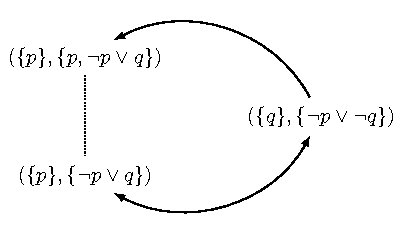
\includegraphics[]{evil_pictures/first_fig.pdf}
%\caption{A fairly simple example}
\label{fig:example2}
}
\subfigure[A more complex example]{
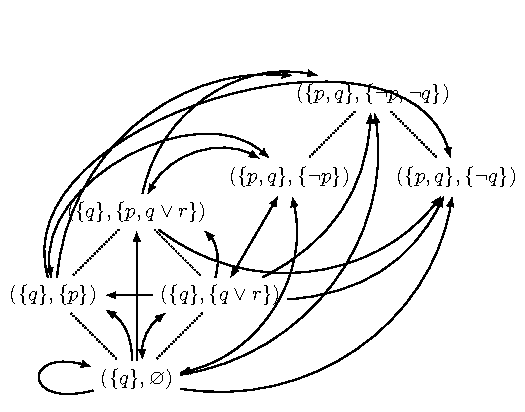
\includegraphics[]{evil_pictures/second_fig.pdf}
\label{fig:example3}
}
\caption{\textsc{EviL} model visualizations}
\end{figure}

Following the modified semantics provided in \S\ref{multi-agent}, the
developments this section will assume multiple agents.
\begin{definition}
  Let $\Phi$ be a set of letters and let $\mathcal{A}$ be a set of agents. 
  A \textbf{Kripke structure} is a state transition system $\mathbb{M}=\langle W^{\mathbb{M}}, R^{\mathbb{M}},
  \sqsubseteq^{\mathbb{M}}, \sqsupseteq^{\mathbb{M}}, V^{\mathbb{M}},
  P^{\mathbb{M}}_{\circlearrowleft} \rangle$ where\footnote{Where
    the context is clear, we shall drop $\mathbb{M}$}:
  \begin{itemizedot}
    \item $W^{\mathbb{M}}$ is a set of worlds    
    \item $R^{\mathbb{M}} : \mathcal{A} \rightarrow \powerset (W \times W)$, $\sqsubseteq^{\mathbb{M}} : \mathcal{A} \rightarrow \powerset (W \times W)$, and $\sqsupseteq^{\mathbb{M}} : \mathcal{A} \rightarrow \powerset (W \times W)$ are
    $\mathcal{A}$-indexed sets of relations\footnote{we shall abbreviate
      $R(X)$, $\sqsubseteq(X)$ and $\sqsupseteq(X)$ as $R(X)$,
      $\sqsubseteq(X)$ and $\sqsupseteq(X)$ as $R_X$, $\sqsubseteq_X$
      and $\sqsupseteq_X$ respectively.}
    \item $V : \Phi \rightarrow \powerset (W)$ is a predicate letter valuation
    \item $P_{\circlearrowleft} : \mathcal{A} \rightarrow \powerset
      (W)$ are sets of worlds indexed by agents
  \end{itemizedot}
  Let $\mathcal{K}_{\Phi, \mathcal{A}, I}$ denote the class of Kripke structures for letters $\Phi$, agents $\mathcal{A}$, and where $W \subseteq I$.
\end{definition}
Kripke semantics given by $(\Vdash) : \mathcal{K}_{\Phi, \mathcal{A}, I} \to I
\rightarrow \text{\tmtextsf{bool}}$ for these models are defined recursively
as usual, granted the exceptional behavior of $P_{\circlearrowleft}$.
\begin{definition}
  Let $\mathbbm{M}$ be in the class $\mathcal{K}_{\Phi, \mathcal{A}, I}$
  \begin{eqnarray*}
    \mathbbm{M}, w \Vdash p & \Longleftrightarrow & w \in V^{\mathbbm{M}}
    (p)\\
    \mathbbm{M}, w \Vdash \phi \rightarrow \psi & \Longleftrightarrow &
    \mathbbm{M}, w \Vdash \phi \text{ implies } \mathbbm{M}, w \Vdash \psi\\
    \mathbbm{M}, w \Vdash \bot & \Longleftrightarrow & \text{False}\\
    \mathbbm{M}, w \Vdash \Box_X \phi & \Longleftrightarrow & \forall v \in
    W^{\mathbbm{M}} . w R^{\mathbbm{M}}_X v \text{ implies } \mathbbm{M}, v
    \Vdash \phi\\
    \mathbbm{M}, w \Vdash \boxminus_X \phi & \Longleftrightarrow & \forall v
    \in W^{\mathbbm{M}} . w \sqsupseteq^{\mathbbm{M}}_X v \text{ implies }
    \mathbbm{M}, v \Vdash \phi\\
    \mathbbm{M}, w \Vdash \boxplus_X \phi & \Longleftrightarrow & \forall v
    \in W^{\mathbbm{M}} . w \sqsubseteq^{\mathbbm{M}}_X v \text{ implies }
    \mathbbm{M}, v \Vdash \phi\\
    \mathbbm{M}, w \Vdash \circlearrowleft_X & \Longleftrightarrow & w \in
    P_{\circlearrowleft}^{\mathbbm{M}} (X)
  \end{eqnarray*}
\end{definition}
Kripke structures can be observe to have a lot less structure than
\tmtextsc{EviL} models.  However, \tmtextsc{EviL} models can be understood as
Kripke structures in disguise.  To illustrate this, observe the following
lemma:
\begin{definition}[$\mho^\Omega$ Translation]
Let $\Omega$ be an \tmtextsc{EviL} model.  Define
  $\mho^{\Omega} \assign \langle \Omega, R^{\Omega},
  \sqsubseteq^{\Omega}, \sqsupseteq^{\Omega}, V^{\Omega},
  P_{\circlearrowleft}^{\Omega} \rangle$, where
  \[ \begin{array}{llll}
       \bullet & \text{$(a, A) R^{\Omega}_X (b, B) \Longleftrightarrow \forall
       \psi \in A_X .b \models \psi$} & \bullet & (a, A)
       \sqsubseteq^{\Omega}_X (b, B) \Longleftrightarrow a = b \text{ and }
       A_X \subseteq B_X\\
       \bullet & (a, A) \sqsupseteq^{\Omega}_X (b, B) \Longleftrightarrow a =
       b \text{ and } A_X \supseteq B_X & \bullet & (a, A) \in
       P_{\circlearrowleft}^{\Omega} (X) \Longleftrightarrow \forall \psi \in
       A_X .a \models \psi
     \end{array} \]
\end{definition}
\begin{lemma}
  \label{tranlemma1} For all $\Omega$ and all $(a, A) \in \Omega$,  $\Omega, (a, A) \VDash
  \phi$ if and only if $\mho^{\Omega}, (a, A) \Vdash \phi$
\end{lemma}
\begin{proof}
  This follows from a straightforward induction on $\phi$.
\end{proof}
The following summarizes the structural properties of
\tmtextsc{EviL} models, when transformed into Kripke structures:
\begin{proposition}\label{evil_models}
  For any \textsc{EviL} model $\Omega$,  $\mho^{\Omega}$ has the following
  properties{\footnote{Note that in this we have that $\{w,v\} \subseteq \powerset \Phi
      \times \powerset \mathcal{L}_0$ in the subsequent discussion}}:
  \begin{myRoman}
    \item\label{pI} $\sqsupseteq^{\Omega}_X$ is reflexive
    \item $\sqsupseteq^{\Omega}_X$ is transitive 
    \item \label{pantisym}$\sqsupseteq^{\Omega}_X$ is anti-symmetric
    \item $w \sqsupseteq^{\Omega}_X v$ if and only if $v
    \sqsubseteq^{\Omega}_X w$
    \item If $w \sqsubseteq^{\Omega}_X v$ then $w \in V (p)$ if and only if $v
    \in V (p)$
    \item \label{pV}$(R^{\Omega}_X \circ \sqsubseteq^{\Omega}_X) \subseteq
    R^{\Omega}_X \subseteq (R^{\Omega}_X \circ \sqsupseteq^{\Omega}_X)$
    \item \label{pVI} $(\sqsubseteq^{\Omega}_Y \circ R^{\Omega}_X) = R^{\Omega}_X =
    (\sqsupseteq^{\Omega}_Y \circ R^{\Omega}_X)$
    \item\label{pVII} $w \in P_{\circlearrowleft}^{\Omega} (X)$ if and only if $w
    R^{\Omega}_X w$
  \end{myRoman}
  \ldots the situation in \ref{pV} can be visualized in
  \ref{fig:commut1}, while \ref{pVI} can be split into
  Figs. \ref{fig:commut2} and \ref{fig:commut3}.
\end{proposition}
\begin{figure}[ht]
\centering
\subfigure[\ref{pV} - $(R^{\Omega}_X \circ \sqsubseteq^{\Omega}_X) \subseteq
R^{\Omega}_X$ and $R^{\Omega}_X \subseteq (R^{\Omega}_X \circ
\sqsupseteq^{\Omega}_X)$ ]{
  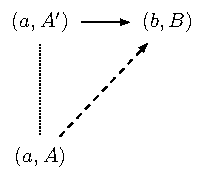
\includegraphics[]{commutative/commutative1.pdf}
%\caption{A fairly simple example}
\label{fig:commut1}
}
\hspace{1cm}
\subfigure[\ref{pVI} - $(\sqsubseteq^{\Omega}_Y \circ R^{\Omega}_X) \subseteq
R^{\Omega}_X$ and \ \ \ \  $R^{\Omega}_X \subseteq
(\sqsupseteq^{\Omega}_Y \circ R^{\Omega}_X)$]{
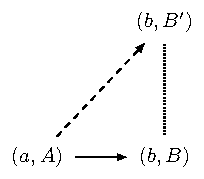
\includegraphics[]{commutative/commutative2.pdf}
\label{fig:commut2}
}
\hspace{1cm}
\subfigure[\ref{pVI} - $(\sqsupseteq^{\Omega}_Y \circ R^{\Omega}_X) \subseteq
R^{\Omega}_X $ and \ \ \ \  $R^{\Omega}_X \subseteq
(\sqsubseteq^{\Omega}_Y \circ R^{\Omega}_X)$]{
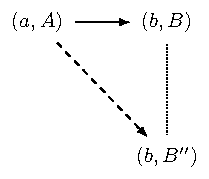
\includegraphics[]{commutative/commutative3.pdf}
\label{fig:commut3}
}
\caption{Visualizations of the relationships in Proposition \ref{evil_models}}
\end{figure}
\begin{proof}
  Everything except \ref{pV} follows directly from the definitions - so we shall only
  demonstrate $R^{\Omega}_X \subseteq R^{\Omega}_X \circ
  \sqsupseteq^{\Omega}_X$.
  
  Suppose that $(a, A) R^{\Omega}_X (b, B)$, then evidently $\forall \psi \in
  A_X .b \models \psi$. 
  Now assume that $(a, A) \sqsupseteq_X^{\Omega} (c,
  C)$.  Then we know that $A_X \supseteq C_X$.
  But then $\forall \psi \in
  C_X .b \models \psi$, so $(c, C) R^{\Omega}_X (b, B)$, which
  suffices to show the claim.
\end{proof}

\begin{definition}
A Kripke structure is called \textsc{EviL} if it makes true the
  above properties \ref{pI} through \ref{pVII} (with the exception of \ref{pantisym}, which is optional).
\end{definition}

These properties are definitive - as shall be demonstrated in \S\ref{Abstract-Completeness}, \tmtextsc{EviL} is
sound and strongly complete for \tmtextsc{EviL} models.

The Kripke semantics also serve to provide proper intuition behind
\tmtextsc{EviL} models. We think of the defined relations given as follows:
\begin{itemizedot}
  \item If $x R^{\Omega}_X y$, then at world $x$ the agent $X$ can imagine $y$
  is true, since $y$ is compatible with what the agent believes 
  \item If $x \sqsubseteq^{\Omega}_X y$, then at world $x$, agent $X$'s
  assumptions (or the experiences they are taking under consideration) are
  contained in her evidence at $y$
\end{itemizedot}
Given this perspective, the proof of \ref{pV} can be understood in the
following way - if the agent assumes fewer things, more things are imaginable,
since it's easier for a world to be incompatible with an agent's evidence.

Finally, while Prop. \ref{evil_models} presents itself as a sort of
representation lemma, the relationship between \textsc{EviL} semantics
and Kripke semantics is not reciprocal.  Not every Kripke model can be
represented as an \textsc{EviL} model.  Example
\ref{not-an-evil-model} presents an elementary example of 
this failure of representation.  It turns on the following
observation:

\begin{lemma}
  For a given \textsc{EviL} model $\mathfrak{M}$, for any
  $\{(a,A),(b,B),(c,C)\} \subseteq \mathfrak{M}$, if $a = b$ then $a
  \models C$ if and only if $b \models C$
\end{lemma}
\begin{proof}
  This is an elementary result in the semantics of propositional logic.
\end{proof}

\begin{example}\label{not-an-evil-model}
Consider a single agent \textsc{EviL} Kripke structure $\mathbb{M}:=\langle W, R,
  \sqsubseteq, \sqsupseteq, V, P \rangle$ where
\begin{bul}
  \item $W := \{w,v\}$
  \item $R := \{(w,v)\}$
  \item $ \sqsubseteq := \sqsupseteq := \{(w,w),(v,v)\}$
  \item $V(p) := \varnothing$ for all $p\in \Phi$
  \item $P := \varnothing$
\end{bul}
\ldots this structure is indicated in Fig. \ref{fig:notevil}.  No
\textsc{EviL} model corresponds to $\mathbb{M}$.
%\end{lemma}
\begin{figure}[ht]
\centering
  
\includegraphics[]{evil_pictures/third_fig.pdf}
%\caption{A fairly simple example}
\label{fig:notevil}
\caption{$\mathbb{M}$ is a Kripke Structure with no \textsc{EviL} representation}
\end{figure}
%\begin{proof}

Observe that the above model makes true the following:

\begin{align}
  \mathbb{M},w & \Vdash \Pos \top \label{notevil:eq1}\\
  \mathbb{M},w & \Vdash \Nec \neg p \textup{ for all $p \in
    \Phi$} \label{notevil:eq4} \\
  \mathbb{M},w & \Vdash \neg p \textup{ for all $p \in \Phi$} \label{notevil:eq2} \\
  \mathbb{M},w & \Vdash \neg \Pos \Pos \top \label{notevil:eq3} 
\end{align}

Armed with these observations, we can assert that it is impossible for
there to be an \textsc{EviL} structure $\mathfrak{M}$ with a world
$(a,A)$ such that $\mathbb{M},w \Vdash \phi$ if and only if
$\mathfrak{M}, (a,A) \VDash \phi$.

For suppose there were, then we could deduce the following facts, using
the observations above:
\begin{mynum}
\item\label{notevil:1} From \eqref{notevil:eq1}, there must be some pair $(b,B)
   \in \mathfrak{M}$ such that $b\models A$.  Hence, $A$ must be
   \emph{consistent}.
\item From \eqref{notevil:eq4}, we know that for the $b$ mentioned in
  \ref{notevil:1}, it must be that $b = \varnothing$ -- this is a
  direct consequence of Lemma \ref{truthiness}, the Truthiness Lemma.
 \item From \eqref{notevil:eq2}, evidently $a = \varnothing$
  \item From \eqref{notevil:eq3}, it must be
    that $a \nmodels A$, since otherwise we would have
    $\mathfrak{M},(a,A) \VDash \Pos \Pos \top$
\end{mynum}
This is absurd... since $a = b = \varnothing$ and $b \models A$
then it must be that $a \models A$. $\lightning$
%\end{proof}
\end{example}

The above one way correspondence is inconvenient - it means that while
\textsc{EviL} only enjoys some features from modal logic, it is denied
others.  Despite this, \textsc{EviL} enjoys \emph{most} of the
benefits of basic modal logic.  Furthermore, even though \textsc{EviL}
is quite formal in nature, it might rightly be considered an
application  of traditional modal logic rather than a novel logic
in of itself.   The novelty of \textsc{EviL} is that it presents semantics
that automatically connect truth and derivability (as expressed in
Theorem \ref{theorem-theorem}, the Theorem Theorem).

%%% Local Variables: 
%%% mode: latex
%%% TeX-master: "evil_philosophy"
%%% End: 
